\section{Convolutional Neural Network Classifier} \label{sec:CNN}
	\pagestyle{mario}
	\sectionauthor{M. Gini \& T. M. Hayden}

CNN is a more advanced architecture than a basic MLP. Similarly to a MLP, it consists of an input and an output layer, as well as several hidden layers. The hidden layers typically consist of convolutional units and fully connected layers. Due to that, CNN are usually much deeper than MLP networks.

CNN typically require significantly more computing power to train. Even though MATLAB supports training on the GPU, some quick maths revealed that our computational resources are insufficient for extensive parameter search on a CNN. A basic CNN is implemented to compare the performance with the MLP.

\subsection{Network Structure}

Since the number of hidden layers in a CNN can be quite large and many different types of layers are available, the number of hyperparameters is even larger than for a MLP classifier. This requires unreasonable amounts of training time. Therefore, this section only presents the final version of our CNN which is found through small trial-and-error tests. It consists of an input layer, convolutional units, fully connected layers and an output layer. The functionality of each layer type is briefly described below.

\begin{itemize}

	\item \textbf{Input Layer}\\
	This layer inputs the raw image data to the network. It also applies data normalization by subtracting the per-pixel mean value over the training dataset. It therefore includes the data preprocessing step.

	\item \textbf{Convolutional Units}\\
	A convolutional unit consists of several layers. The first layer is always the \textit{convolutional layer}. It has parameters for filter size and depth, which control the size and number of the feature maps the layer is analyzing. This layer is followed by a \textit{batch normalization layer} which normalizes the activations and gradients propagating through a network, making network training an easier optimization problem.

	Then, a \textit{rectified linear unit} (ReLU) follows. This is a nonlinear activation function very commonly used in CNN. Finally, a convolutional unit has a \textit{max-pooling layer} that reduces the spatial size of the feature map. This removes redundant spatial information. As a consequence, the number of layers can be increased without increasing the amount of computation time per layer. A max-pooling layer simply returns the maximum values of rectangular regions of inputs.

	\item \textbf{Fully Connected Layers}\\
	Fully connected layers are usually employed between the convolutional layers and the output layer. As the name suggests, they are fully connected to all neurons in the preceding layer. It therefore combines all the features learned by the previous layers across the image to identify larger patterns.

	\item \textbf{Output Layers}\\
	The output layer consists of a softmax layer as described in Section \ref{subsec:setup} together with a classification layer which simply chooses the class that achieved the highest probability by the softmax layer.

\end{itemize}

Table \ref{Tab:CNNStructure} shows the implementation of our final CNN in MATLAB. Three convolutional units are employed with a filter size of $3\time3$ pixels and a varying number of filters. For the max-pooling layers, a filter size of $2\times2$ pixels is used. Two fully connected layers and the output layers complete our CNN architecture.

\begin{table}[h]
	\begin{center}
		\begin{tabular}{||c | c||}
			\hline
			\textbf{Layer Type}& \textbf{MATLAB Implementation} \\ [0.5ex]
			\hline
			Input Layer& Imageinputlayer(\lbrack32,32,2\rbrack)\\
			\hline
			 & convolution2dLayer(3,16,'Padding',1) \\
			First& batchNormalizationLayer\\
			Convolutional Unit& reluLayer\\
			 & maxPooling2dLayer(2,'Stride',2)\\
			\hline
			 & convolution2dLayer(3,32,'Padding',1)\\
			Second& batchNormalizationLayer\\
			Convolutional Unit& reluLayer\\
			 & maxPooling2dLayer(2,'Stride',2)\\
			\hline
			 & convolution2dLayer(3,64,'Padding',1)\\
			Third& batchNormalizationLayer\\
			Convolutional Unit& reluLayer\\
			& maxPooling2dLayer(2,'Stride',2)\\
			\hline
			Fully Connected& fullyConnectedLayer(10)\\
			Layers& fullyConnectedLayer(10)\\
			\hline
			Output& softmaxLayer\\
			Layers& classificationLayer\\
			\hline

		\end{tabular}
		\caption{The CNN structure as implemented in MATLAB.}
		\label{Tab:CNNStructure}
	\end{center}
\end{table}
\FloatBarrier
\subsection{Network Training Results}

MATLAB has introduced a convenient CNN training GUI in the R2017b release. Figure \ref{fig:CNNTrain} shows a screenshot of the GUI that allows to observe the training progress. Together with the GUI, several applications have been updated as well. For example, any GPU is automatically detected and used for training. Our CNN training takes place on a single GPU of type NVIDIA GeForce GT 640M. The training of a single configuration takes around \SI{20}{\minute}. The architecture described in Table \ref{Tab:CNNStructure} is found to obtain a test accuracy of 74.22\%. This is considerably better than the MLP even though it is not yet a fully optimized CNN architecture.

\begin{figure}[h!]
	\centering
	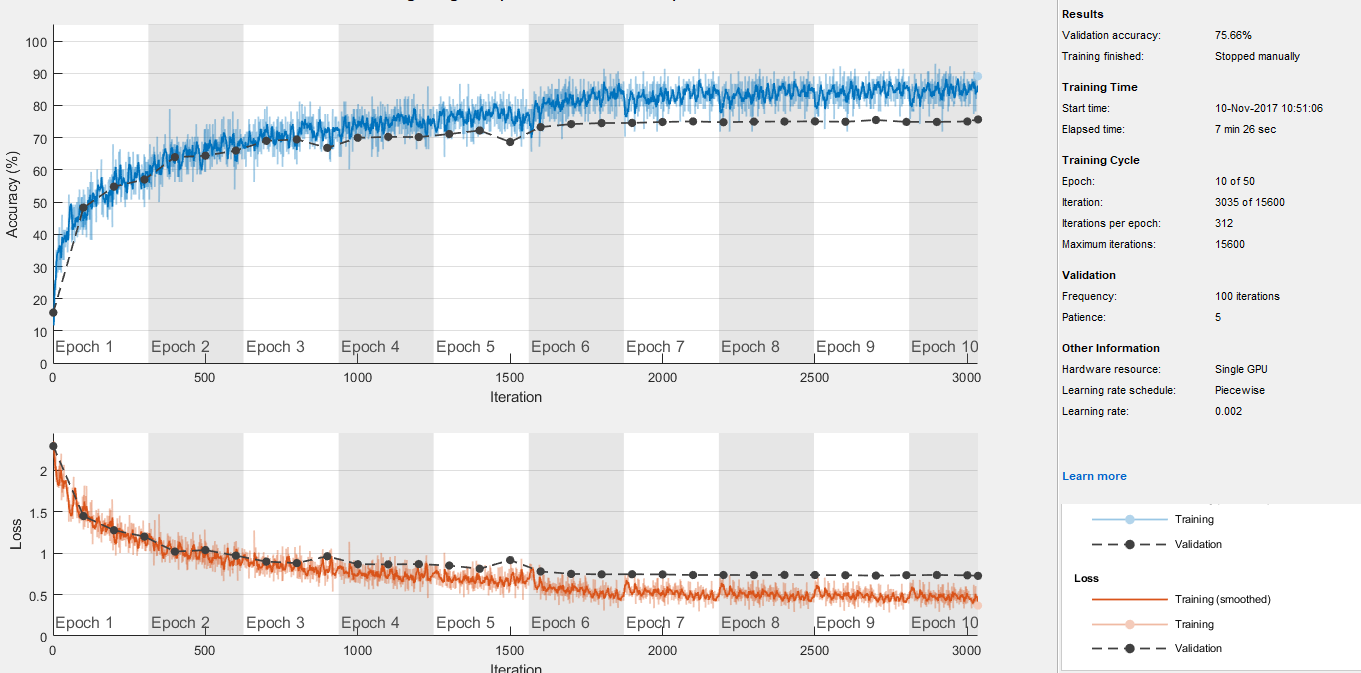
\includegraphics[width=\textwidth]{images/CNNTrain}
	\caption{Screenshot of MATLAB GUI for training a CNN. The blue \& red curves represent performance on the training dataset, while the black line represents the performance on the validation dataset.}
	\label{fig:CNNTrain}
\end{figure}

Figure \ref{fig:CNNConfusion} shows the confusion matrix for the CNN. The most likely misclassifications are similar to that of the MLP, e.g. the misclassification between cats and dogs is significantly higher than between other classes.

\begin{figure}[h!]
	\centering
	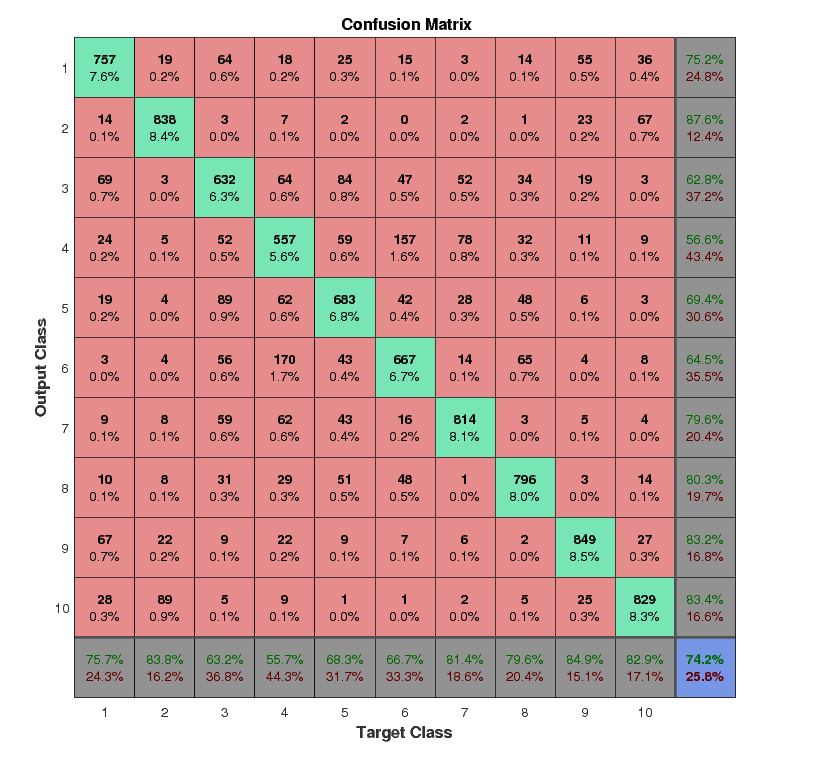
\includegraphics[width=\textwidth]{images/Confusion_MatrixCNN.png}
	\caption{Confusion matrix for the final CNN.}
	\label{fig:CNNConfusion}
\end{figure}
\FloatBarrier
